This chapter introduces time simulation algorithms for Hamiltonian \ref{eq:HeisenbergHamiltonian}. First a trotterization scheme is introduced, and its advantages are discussed for simulating certain types of graphs or lattices. Relations between discretization step, evolution time and evolution error are computed and discussed in order to establish disadvantages of execution on current (noisy) quantum devices. Then, three possible implementation strategies are introduced: 1) a direct transpilation of includes proposed by Las Heras et. al. \cite{HubbardSimulLasHeras}, 2) a basis-efficient transpilation relying on commutation properties of local Hamiltonians \footnote{The work was performed at early stages independently of that on \cite{BellUniversalCartan}. However, the insights are identical and thus the author is compelled to refer to this previous work. It is clear, however, that the mentioned reference considers the problem of universal two qubit gates which, albeit related to the specific problem of the present dissertation, is a quite different approach. This dissertation uses the results derived to solve a specific time evolution problem with potential application to specific areas of solid state physics and physical chemistry.}, and 3) a pulse-efficient transpilation based on cross-resonance interaction. Finally, the three algorithms are tested using a three-qubit Hamiltonian. Single-qubit Pauli expected value evolution and probability density evolution as qualitative indicators, whereas probability density fidelity and state fidelity are used as quantitative indicators.

\section{Trotterization And Time Evolution}
\label{sec:MainTrotterScheme}

  Consider the multiple spin Hamiltonian

  \begin{equation}
    \hat{H} = \sum_{\langle i,j \rangle} J_{ij}^{(X)} \hat{X}_i \hat{X}_j + J_{ij}^{(Y)} \hat{Y}_i \hat{Y}_j + J_{ij}^{(Z)} \hat{Z}_i \hat{Z}_j + \sum_i h_i^{(X)} \hat{X}_i + h_i^{(Y)} \hat{Y}_i + h_i^{(Z)} \hat{Z}_i,
    \label{eq:HeisenbergHamiltonian2}
  \end{equation}

  \noindent defined over an arbitrary graph. The shape already suggests that the Hamiltonian above can be decomposed in local interactions of the shape

  \begin{gather}
    \hat{H}_{ij} = J_{ij}^{(X)} \hat{X}_i \hat{X}_j + J_{ij}^{(Y)} \hat{Y}_i \hat{Y}_j + J_{ij}^{(Z)} \hat{Z}_i \hat{Z}_j, \\
    \hat{H}_{i} = h_i^{(X)} \hat{X}_i + h_i^{(Y)} \hat{Y}_i + h_i^{(Z)} \hat{Z}_i,
    \label{eq:HamiltonianDecomposition}
  \end{gather}

  \noindent such that

  \begin{equation}
    \hat{H} = \sum_{\langle i,j \rangle} \hat{H}_{ij} + \sum_i \hat{H}_i.
  \end{equation}

  This leads to a direct second order trotterization of the shape

  \begin{equation}
    \mathrm{e}^{-\mathrm{i}\hat{H}\Delta t} \approx \prod_{\langle i,j \rangle} \mathrm{e}^{-\mathrm{i}\hat{H}_{i,j}\Delta t} \prod_{i} \mathrm{e}^{-\mathrm{i}\hat{H}_i \Delta t} + \mathcal{O}(\Delta t^2).
    \label{eq:HamiltonianTrotterization}
  \end{equation}

  In general, interactions associated to disjoint edges commute, and thus can be simulated simultaneously. Hence, an advantage of this approach to time evolution is that by partitioning the graph on sets of mutually disjoint sets, several terms can be implemented in parallel on actual quantum devices. This approach is implemented in the present work, and discussed further on the appendix. This parallelism is illustrated for a spin chain in figure \ref{fig:spinChainCircuit}. It can be noticed that the circuit depth of the trotter step of three or more spins with chain topology is independent of the number of spins. As a result, time complexity only increases with the desired time discretization, which correlates with the error in the time simulation approximation. 
  
  Another interesting feature, as shown in figure \ref{fig:spinChainCircuit}, is that it is possible to perform third order time evolution using the first iteration of Suzuki-Trotter scheme with roughly the sme time complexity as the second order trotterization. This, clearly, in the case where no external local fields are present in the model Hamiltonian, and the graph corresponds to a chain. To illustrate the point more precisely, consider the Hamiltonian

  \begin{equation}
    \hat{H} = \sum_{i=0}^{N-2} \hat{H}_{i,i+1},
    \label{eq:ChainHamiltonian}
  \end{equation}

  \noindent where $\hat{H}_{i,j}$ is defined as on equation \ref{eq:HamiltonianDecomposition}. It is quite straightforward to see the that the second order evolution corresponds to the approximation

  \begin{equation}
    \mathrm{e}^{-\mathrm{i}\hat{H}\Delta t} \approx \prod_{i \text{ even}} \mathrm{e}^{-\mathrm{i}\hat{H}_{i,i+1}t} \prod_{i \text{ odd}} \mathrm{e}^{-\mathrm{i}\hat{H}_{i,i+1}t} + \mathcal{O}(\Delta t^2).
    \label{eq:HamiltonianTrotterization}
  \end{equation}

  For this particular system, denote

  \begin{gather}
    \hat{A}(\Delta t) = \prod_{i \text{ even}} \mathrm{e}^{-\mathrm{i}\hat{H}_{i,i+1}t} \\
    \hat{B}(\Delta t) = \prod_{i \text{ odd}} \mathrm{e}^{-\mathrm{i}\hat{H}_{i,i+1}t}
    \label{eq:ChainOpsTrotter}
  \end{gather}

  \noindent such that

  \begin{equation}
    \mathrm{e}^{-\mathrm{i}\hat{H}\Delta t} \approx \hat{A}(\Delta t) \hat{B}(\Delta t) + \mathcal{O}(\Delta t^2)
    \label{eq:HamiltonianTrotterization}
  \end{equation}

  Simulation over a time $t = M \Delta t$ yields

  \begin{equation}
    \mathrm{e}^{-\mathrm{i}\hat{H}t} \approx \bigg( \hat{A}(\Delta t) \hat{B}(\Delta t) \bigg)^{M}.
    \label{eq:HamiltonianTrotterization}
  \end{equation}

  The third order scheme may be implemented using Suzuki-Trotter zeroth order evolution (eq. \ref{eq:Suzuki0}), yielding the following finite time approximation

  \begin{equation}
    \begin{aligned}
      \mathrm{e}^{-\mathrm{i}\hat{H}t} \approx & \bigg( \hat{A}(\Delta t/2) \hat{B}(\Delta t) \hat{A}(\Delta t/2) \bigg)^{M} \\
    = &  \hat{A}(\Delta t/2) \bigg( \hat{B}(\Delta t) \hat{A}(\Delta t) \bigg)^{M-1} \hat{B}(\Delta t) \hat{A}(\Delta t/2) \\
    = & \hat{A}(\Delta t/2) \hat{B}(\Delta t) \bigg( \hat{A}(\Delta t) \hat{B}(\Delta t) \bigg)^{M-1} \hat{A}(\Delta t/2).
    \label{eq:HamiltonianTrotterization}
    \end{aligned}
  \end{equation}

  It can be seen that the \textit{power} operator (the one with a power in the approximation unitary) on each scheme can be implemented in the same fashion on a quantum circuit. Hence, both second order and third order schemes have roughly the same time complexity when implemented on quantum devices. This optimization is taken into account during implementation on IBM Quantum backends.
  
  \begin{figure}
    \centering
    \begin{quantikz}
        & \gate[wires=2]{\mathrm{e}^{-\mathrm{i}\hat{H}_{0,1}\Delta t}} & \qw & \gate{\mathrm{e}^{-\mathrm{i}\hat{H}_{0}\Delta t}} & \qw \\
        & \qw & \gate[wires=2]{\mathrm{e}^{-\mathrm{i}\hat{H}_{1,2}\Delta t}} & \gate{\mathrm{e}^{-\mathrm{i}\hat{H}_{1}\Delta t}} & \qw \\
        & \gate[wires=2]{\mathrm{e}^{-\mathrm{i}\hat{H}_{2,3}\Delta t}} & \qw & \gate{\mathrm{e}^{-\mathrm{i}\hat{H}_{2}\Delta t}} & \qw \\
        & \qw & \gate[wires=2]{\mathrm{e}^{-\mathrm{i}\hat{H}_{3,4}\Delta t}} & \gate{\mathrm{e}^{-\mathrm{i}\hat{H}_{1}\Delta t}} & \qw \\
        & \qw & \qw  &      \gate{\mathrm{e}^{-\mathrm{i}\hat{H}_{4}\Delta t}} & \qw
    \end{quantikz}
    \caption{Trotter step for simulating a spin chain. Notice that spin-spin terms that do not share a graph point can be evolved in parallel. A greedy algorithm can be used to determine a possible, if not optimal, scheme for simulating spin-spin interactions on parallel.}
    \label{fig:spinChainCircuit}
\end{figure}

\section{Circuit implementations}
\label{sec:MainCircuits}
  
  On chapter \ref{chap:qc}, some networks for simulating time evolution of the two-qubit Hamiltonian were introduced (see fig. \ref{fig:salathe-includes}). In this section, three possible transpiled includes are introduced. Those implement the single qubit and two qubit operators on equation \ref{eq:HamiltonianDecomposition}. The single qubit operators are implemented in the same way on all three alternatives. Each circuit differs from the others on the implementation of the two spin operators. The first alternative is a direct basis transpilation, based on the controlled phase gate. The second alternative is one that takes advantage of the commutation properties of the local two spin Hamiltonian. This alternative was derived mostly independently from \cite{BellUniversalCartan} at early stages of the present work. However,a thorough discussion of the insights required to derive this circuit is included. The last option is a cross resonance based implementation as discussed on chapter \ref{chap:qc}.

  \subsection{Simulation of field interaction}
  \label{subsec:fieldInteractionCircuit}

    To simulate evolution under Hamiltonian \ref{eq:HamiltonianDecomposition}, a direct approach would be to us te definition of single qubit rotations, and implement a second order trotterization scheme as illustrated on figure \ref{fig:directSimulationFieldSpin}. However, exact simulation of this model is possible by rotating the Bloch sphere main axes so that the external field points to the $\hat{z}$ direction. This can be done by the operator

    \begin{equation}
      \hat{U}_{\theta,\phi} = \begin{bmatrix}
        \cos(\frac{\theta}{2}) & \sin(\frac{\theta}{2}) \\
        \mathrm{e}^{\mathrm{i}\phi}\sin(\frac{\theta}{2}) & -\mathrm{e}^{\mathrm{i}\phi}\cos(\frac{\theta}{2}),
      \end{bmatrix}
      \label{eq:UGate}
    \end{equation}

    \noindent where $\theta$ and $\phi$ are defined by the spherical representation of the external field (see eq. \ref{eq:PolarRepresentation}):

    \begin{gather}
      h^2 =  (h_i^{(x)})^2 + (h_i^{(y)})^2 + (h_i^{(z)})^2 ,\\
      h_i^{(x)} = h \sin(\theta)\cos(\phi), \\
      h_i^{(y)} = h \sin(\theta)\sin(\phi), \\
      h_i^{(z)} = h \cos(\theta).
      \label{eq:PolarRepresentation}
    \end{gather}

    This approach is illustrated on figure \ref{fig:rotatedSimulationFieldSpin}. Therefore, at the same computational cost, this interaction can be simulated exactly by the former algorithm.

    \begin{figure}
    \centering
    \begin{subfigure}[b]{1.0\textwidth}
        \centering
        \caption{}
        \begin{quantikz}
            & \gate{\hat{R}_{\hat{x},2h_i^{(X)}\Delta t}} & \gate{\hat{R}_{\hat{y},2h_i^{(Y)}\Delta t}} & \gate{\hat{R}_{\hat{z},2h_i^{(Z)}\Delta t}} & \qw
        \end{quantikz}
        \label{fig:directSimulationFieldSpin}
    \end{subfigure}
    \begin{subfigure}[b]{1.0\textwidth}
        \centering
        \caption{}
        \begin{quantikz}
            & \gate{\hat{U}_{\theta,\phi}^{\dagger}} & \gate{\hat{R}_{\hat{z},2h \Delta t}} & \gate{\hat{U}_{\theta,\phi}} & \qw
        \end{quantikz}
        \label{fig:rotatedSimulationFieldSpin}
    \end{subfigure}
    \caption{(a) Direct trotterization of field-spin interaction for small time interval $\Delta t$. (b) Exact simulation by rotating the Bloch sphere reference frame to the external field direction.}
    \label{fig:directTrotterizationFieldSpin}
\end{figure}

  \subsection{Simulation of Two-spin Interaction}
  \label{subsec:TwoSpinCircuits}

    The simpler spin-spin Hamiltonian

    \begin{equation}
      \hat{H}_{ij} = J_{ij}^{(X)} \hat{X}_i \hat{X}_j + J_{ij}^{(Y)} \hat{Y}_i \hat{Y}_j + J_{ij}^{(Z)} \hat{Z}_i \hat{Z}_j
      \label{eq:SpinSpin}
    \end{equation}

    \noindent is simulated using IBM Quantum device's universal set, or cross resonance pulses. This is the most computationally expensive part of the evolution scheme. As may be seen on figure \ref{fig:echoedPulseQiskit}, the most time consuming processes are simulating two qubit interactions. In consequence, reducing the number and duration of CNOT gates or cross resonance pulses on the evolution algorithm is crucial for obtaining high fidelity results. Here, a first network that performs direct transpilation of circuit \ref{fig:heras-hubbard} is presented. It will be used as a control case, since non-optimized transpilations would yield this network for simulating the Hamiltonian \cite{Qiskit}. A basis efficient circuit is introduced, and its mathematical and physical insights are discussed \cite{BellUniversalCartan}. Finally, the pulse efficient network proposed on \cite{RXZPulseEfficient} is revisited.
    
    \subsubsection{Direct transpilation circuit}
    \label{subsubsec:DirectTranspilationCircuit}

      To adapt circuit \ref{fig:heras-hubbard} for IBM Quantum devices, it is helpful to note that

      \begin{equation}
        \mathrm{e}^{-\mathrm{i}\phi \hat{Z}_i \otimes \hat{Z}_j} = \cos(\frac{\phi}{2}) - \mathrm{i}\sin(\frac{\phi}{2}) \hat{Z}_i \otimes \hat{Z}_j = 
        \begin{bmatrix}
          \mathrm{e}^{-\mathrm{i}\frac{\phi}{2}} & 0 & 0 & 0 \\
          0 & \mathrm{e}^{\mathrm{i}\frac{\phi}{2}} & 0 & 0 \\
          0 & 0 & \mathrm{e}^{\mathrm{i}\frac{\phi}{2}} & 0 \\
          0 & 0 & 0 & \mathrm{e}^{-\mathrm{i}\frac{\phi}{2}}.
        \end{bmatrix}
        \label{eq:expZZ}
      \end{equation}

      By the definition of CNOT gate, and single-qubit gates (see chap. \ref{chap:qc}), it follows that this operator can be implemented by the circuit on figure \ref{fig:directTrotterSpinZZ}. A direct way to simulate the $XX$ interaction term is to note that

      \begin{equation}
        \hat{H}^{\otimes 2} \mathrm{e}^{-\mathrm{i}\phi \hat{Z}_i \otimes \hat{Z}_j} \hat{H}^{\otimes 2} = \mathrm{e}^{-\mathrm{i}\phi \hat{X}_i \otimes \hat{X}_j},
        \label{eq:Z2X}
      \end{equation}

      \noindent where $\hat{H}$ means the Hadamard gate, not the target Hamiltonian. This follows from the observation that $\hat{H}\hat{Z}\hat{H} = \hat{X}$. In a similar fashion, it is possible to implement the $YY$ interaction by noticing that

      \begin{equation}
        \Big(\hat{R}_{\hat{z}, \pi/2}^{\dagger}\hat{H}\Big)\hat{Z}\Big(\hat{R}_{\hat{z}, \pi/2}^{\dagger}\hat{H}\Big)^{\dagger} = \hat{Y}.
        \label{eq:Z2Y}
      \end{equation}

      \begin{figure}
    \centering
    \begin{subfigure}[b]{1.0\textwidth}
        \centering
        \caption{}
        \begin{quantikz}
            & \ctrl{1} & \qw & \ctrl{1} & \qw \\
            & \targ{}  & \gate{\hat{R}_{\hat{z}, \phi}} & \targ{} & \qw\\
        \end{quantikz}
        \label{fig:directTrotterSpinZZ}
    \end{subfigure}
    \begin{subfigure}[b]{1.0\textwidth}
        \centering
        \caption{}
        \begin{quantikz}
            & \gate{H} & \ctrl{1} & \qw & \ctrl{1} & \gate{H} & \qw \\
            & \gate{H} & \targ{}  & \gate{\hat{R}_{\hat{z}, \phi}} & \targ{} & \gate{H}& \qw\\
        \end{quantikz}
        \label{fig:directTrotterSpinXX}
    \end{subfigure}
    \begin{subfigure}[b]{1.0\textwidth}
        \centering
        \caption{}
        \begin{quantikz}
            & \gate{\hat{R}_{\hat{z}, \pi/2}^{\dagger}} & \gate{H} & \ctrl{1} & \qw & \ctrl{1} & \gate{H} & \gate{\hat{R}_{\hat{z}, \pi/2}} & \qw \\
            & \gate{\hat{R}_{\hat{z}, \pi/2}^{\dagger}} & \gate{H} & \targ{}  & \gate{\hat{R}_{\hat{z}, \phi}} & \targ{} & \gate{H} & \gate{\hat{R}_{\hat{z}, \pi/2}} & \qw\\
        \end{quantikz}
        \label{fig:directTrotterSpinYY}
    \end{subfigure}
    \caption{(a) Implementation of two-spin $ZZ$ interaction using IBM Quantum's universal set. (b) Implementation of $XX$ interaction using basis rotation. (c) Implementation of $YY$ interaction using the same technique as in (b).}
    \label{fig:directTrotterSpinSpin}
\end{figure}

      This leads to a straightforward algorithm for simulating spin-spin interaction that uses 6 CNOT gates, and 15 single-qubit rotations. 
    
    \subsubsection{Basis efficient circuit}
    \label{subsubsec:BasisEfficientCircuit}

      This gate count can be reduced further by considering the commutation relations between the operators that constitute the spin-spin interaction Hamiltonian

      \begin{equation}
        [\hat{X}_i\hat{X}_j, \hat{Z}_i\hat{Z}_j] = [\hat{Y}_i\hat{Y}_j, \hat{Z}_i\hat{Z}_j] = 0.
        \label{eq:CommutationRelations}
      \end{equation}

      From basic quantum mechanics, there exists a common basis in which time evolution under hamiltonian \ref{eq:SpinSpin} implies appending global phases via single qubit rotations around $\hat{z}$ axis, and less two-qubit operations. This basis is straightforward to find by noticing that the \textit{total spin} operator

      \begin{equation}
        \hat{S}^2 = 6 + 2\Big(\hat{X}_i\hat{X}_j + \hat{Y}_i\hat{Z}_j + \hat{Z}_j\Big) 
        \label{eq:TotalSpin}
      \end{equation}

      \noindent commutes with the spin-spin interaction Hamiltonian. From elementary quantum physics, it is known that the eigenstates of such operator are the singlet and triplet states \cite{Beck}. By mapping quantum bit value to spin value directly, it can be readily seen that the singlet and triplet states correspond exactly to the \textit{Bell states} defined on equations \ref{eq:BellBasis}. By considering that

      \begin{gather}
        \hat{X}_i\hat{X}_j \ket{\Phi^{\pm}} = \pm\ket{\Phi^{\pm}}, \\
        \hat{Y}_i\hat{Y}_j \ket{\Phi^{\pm}} = \mp\ket{\Phi^{\pm}}, \\
        \hat{Z}_i\hat{Z}_j \ket{\Phi^{\pm}} = \ket{\Phi^{\pm}},
        \label{eq:PhiBellBasisOps}
      \end{gather}

      \begin{gather}
        \hat{X}_i\hat{X}_j \ket{\Psi^{\pm}} = \pm\ket{\Psi^{\pm}}, \\
        \hat{Y}_i\hat{Y}_j \ket{\Psi^{\pm}} = \pm\ket{\Psi^{\pm}}, \\
        \hat{Z}_i\hat{Z}_j \ket{\Psi^{\pm}} = -\ket{\Psi^{\pm}},
        \label{eq:PsiBellBasisOps}
      \end{gather}

      \noindent it is possible to obtain the energies of the Hamiltonian:

      \begin{gather}
        \hat{H}_{ij} \ket{\Psi^{\pm}} = \bigg(-J_{ij}^{(Z)} \pm (J_{ij}^{(X)} + J_{ij}^{(Y)})\bigg) \ket{\Psi^{\pm}}, \\
        \hat{H}_{ij} \ket{\Phi^{\pm}} = \bigg(J_{ij}^{(Z)} \pm (J_{ij}^{(X)} - J_{ij}^{(Y)})\bigg) \ket{\Phi^{\pm}}.
        \label{eq:SpinSpinEnergies}
      \end{gather}

      To each term $J_{ij}^{(X)}$, $J_{ij}^{(Y)}$, $J_{ij}^{(Z)}$, it is possible to assign a phase $\phi_{xx}$, $\phi_{yy}$, $\phi_{zz}$. Those are defined as follows

      \begin{gather}
        \phi_{xx} = 2 J_{ij}^{(X)} \Delta t, \\
        \phi_{yy} = -2 J_{ij}^{(Y)} \Delta t, \\
        \phi_{zz} = 2 J_{ij}^{(Z)} \Delta t,
        \label{eq:SpinSpinPhases}
      \end{gather}
      
      \noindent where $\Delta t$ is the time interval to be simulated. A quantum circuit representing this approach to evolution is presented on figure \ref{fig:abelianTrotterSpinSpin}. Main stages are separated by slices, which correspond to:

      \begin{enumerate}
        \item Basis change from computational to Bell.
        \item Append $\phi_{xx}$ and $\phi_{zz}$ phases.
        \item Shuffle the basis to append $\phi_{yy}$ phase.
        \item Return to ordered Bell basis
      \end{enumerate}

      In the first stage, the Bell basis is mapped according to

      \begin{gather}
        \ket{\Phi^{+}} \rightarrow \ket{00}, \\
        \ket{\Phi^{-}} \rightarrow \ket{01}, \\
        \ket{\Psi^{+}} \rightarrow \ket{10}, \\
        \ket{\Psi^{-}} \rightarrow \ket{11}. 
      \end{gather}

      From equations \ref{eq:SpinSpinEnergies}, it may be noted that $xx$ phase correlates to the less significant bit, while $zz$ phase correlates to the most significant bit. Also, $yy$ phase correlates to the parity of the mapped computational basis state, hence the need of a CNOT gate. The last part undoes the CNOT gate action on the previous step, and returns to the Bell basis. The direct way to perform the last step is illustrated on figure \ref{fig:abelianTrotterSpinSpin}(a). A more clever approach relies on the following equalities (up to global state phases)

      \begin{gather}
        \ket{\Phi^{+}} = \frac{1}{\sqrt{2}}(\ket{00} + \ket{11}) = \frac{1}{\sqrt{2}}(\ket{+\mathrm{i},-\mathrm{i}} + \ket{-\mathrm{i},+\mathrm{i}}), \\
        \ket{\Phi^{-}} = \frac{1}{\sqrt{2}}(\ket{00} - \ket{11}) = \frac{1}{\sqrt{2}}(\ket{+\mathrm{i},+\mathrm{i}} + \ket{-\mathrm{i},-\mathrm{i}}), \\
        \ket{\Psi^{+}} = \frac{1}{\sqrt{2}}(\ket{01} + \ket{10}) = \frac{1}{\sqrt{2}}(\ket{+\mathrm{i},+\mathrm{i}} - \ket{-\mathrm{i},-\mathrm{i}}), \\
        \ket{\Psi^{-}} = \frac{1}{\sqrt{2}}(\ket{01} - \ket{10}) = \frac{1}{\sqrt{2}}(\ket{+\mathrm{i},-\mathrm{i}} - \ket{-\mathrm{i},+\mathrm{i}}), 
        \label{eq:bellOnYBasis}
      \end{gather}

      \noindent where the single qubit states $\{\ket{+\mathrm{i}}, \ket{+\mathrm{i}}\}$ are defined as on chapter \ref{chap:qc}, and correspond to the $\hat{Y}$ eigenstates. The shuffling stage that appends $yy$ phase actually permutes states $\ket{\Psi^{-}}$ and $\ket{\Psi^{+}}$ of the Bell basis. It is now easy to see that by performing single qubit rotations that are equivalent to the mappings (where the subindex corresponds to qubits 0 and 1, respectively)

      \begin{gather}
        \ket{0}_0 \rightarrow \ket{-\mathrm{i}}_0, \\
        \ket{1}_0 \rightarrow -\mathrm{i}\ket{+\mathrm{i}}_0, \\
        \ket{0}_1 \rightarrow \ket{+\mathrm{i}}_1, \\
        \ket{1}_1 \rightarrow \mathrm{i}\ket{-\mathrm{i}}_1, \\
        \label{eq:localBellShuffling}
      \end{gather}

       \noindent it is possible to perform the desired reordering without using an additional CNOT gate. Such procedure is illustrated on figure \ref{fig:abelianTrotterSpinSpin}(b). On the last state, the computational basis is mapped back to the Bell basis, and the reordering is performed on the Bell basis using local rotations that correspond to transformation \ref{eq:localBellShuffling}. As a result, the number of expensive CNOT gates has been halved with respect to the direct transpilation circuit.

      \begin{figure}
    \centering
    \begin{quantikz}
        & \ctrl{1} & \gate{H} & \gate{\hat{R}_{\hat{z}, \phi_{xx}}} & \ctrl{1}  & \qw                                 & \ctrl{1} & \gate{H} & \ctrl{1} & \qw \\
        & \targ{}  & \qw      & \gate{\hat{R}_{\hat{z}, \phi_{zz}}} & \targ{}  & \gate{\hat{R}_{\hat{z}, \phi_{yy}}} & \targ{}  & \qw      & \targ{}  & \qw \\
    \end{quantikz}
    \caption{Implementation of spin-spin interaction using abelian groups. The first and last two stages perform a change of basis to Bell basis from computational basis. Interaction phases are appended according to the energy values (see eq. \ref{eq:SpinSpinPhases}).}
    \label{fig:abelianTrotterSpinSpin}
\end{figure}

    \subsection{Pulse efficient implementation}
    \label{subsubsec:PulseEfficientCircuit}

      On subsection \ref{subsec:EchoedCrossResonance}, a pulse schedule, introduced in \cite{RXZPulseEfficient}, was presented as an efficient alternative for implementing the unitary operators

      \begin{equation}
        \hat{U}(\alpha, \beta, \gamma) = \mathrm{e}^{-\mathrm{i}(\alpha\hat{X}\hat{X} + \beta\hat{Y}\hat{Y} + \gamma\hat{Z}\hat{Z})}
        \label{eq:CartanDecomp2}.
      \end{equation}

      It can be readily seen that the relations

      \begin{gather}
        \alpha = J_{xx} \Delta t, \\
        \beta = J_{yy} \Delta t, \\
        \gamma = J_{zz} \Delta t,
      \end{gather}

      \noindent yield a unitary that exactly performs time evolution under the two-spin interaction Hamiltonian. The single qubit rotations used on the network representation \ref{fig:PulseEffcientCartanCircuit} profit the relations between Pauli operators stated on equations \ref{eq:Z2X} and \ref{eq:Z2Y}. This algorithm has a slightly different nature than those presented previously. The former two use a particular basis to implement a quantum algorithm that can run on any universal device, regardless of the underlying architecture. The one discussed here, on the other hand, is specifically calibrated for IBM Quantum devices using Qiskit SDK and the pulse scaling technique implemented on \cite{RXZPulseEfficient}.

\section{Comparison and Benchmark: Methodology}
\label{sec:Methodology}

  In general, time simulation of a quantum system has at least two requirements: 1) that the state after evolution resembles within given error bounds the actual target state, and 2) that expected values of interesting observables can be extracted within given error bounds. In the present work, those two requirements are assessed by considering expected value time evolution, probability density (pdf) time evolution, and target probability density fidelity. In this section, the fundamental methods for implementing experiments on quantum devices, measuring observables and computing simulation fidelities are discussed. A benchmark system with Hamiltonian

  \begin{equation}
    \hat{H} = \sum_{i=0}^{1}\Bigg(\hat{X}_i\hat{X}_{i+1} + \hat{Y}_i\hat{Y}_{i+1} + \hat{Z}_i\hat{Z}_{i+1} \Bigg)
    \label{eq:BenchmarkHamiltonian}
  \end{equation}

  \noindent is used for simulation on \textit{ibmq jakarta}. The three proposed schemes discussed on previous sections will be benchmarked by computing the metric mentioned above, for this particular system \footnote{In principle, a larger system could be simulated. However, direct pulse control using the methods proposed on \cite{RXZPulseEfficient} depends on the connectivity if quantum devices. \textit{ibmq jakarta} only supports this type of control on a set of three qubits. Hence the constraints for comparison between the propsed algorithms.}. As a control case, a Qiskit's QASM simulator is used to perform time evolution, since it emulates fault-tolerant quantum computation. This base case will be used for comparing the results obtained by performing the experiment on actual quantum devices and further analysis and discussion.

  \subsection{Measurement of observables}
  \label{subsec:MeasurementMethods}

    Consider the set of of Pauli tensor product operators defined on a space of $N$ qubits. Each of this operators can be mapped to the set of strings whose characters indicate the Pauli operator that acts on the corresponding qubit. For instance,

    \begin{equation}
      \hat{XXI} = \hat{I} \otimes \hat{X} \otimes{X},
    \end{equation}

    \noindent indicating that the operator acts on a 3-qubit space, and applies and identity gate on the third qubit, while applying an $X$ gate on the first two. It is a well known fact that the set of Pauli tensor product operators constitute a basis for the space of operators defined on an $N$-qubit system's Hilbert space \cite{Nielsen, Strini}. Hence, any operator in that space has the expansion
    
    \begin{equation}
      \hat{O} = \sum_{P} c_P \hat{P}
    \end{equation}

    \noindent where $P$ is a Pauli tensor product operator. This fact yields a direct approach towards measuring expected value of operators. If the expected value of Pauli tensors can be measured, then linearity yields the expected value of any $N$-qubit operator. Now, by default, experiments performed on IBM's quantum devices produce the expected value of the Pauli tensor $\otimes^{N} \hat{Z}$. As a result, by applying local rotations to the qubits according to equations \ref{eq:Z2X} and \ref{eq:Z2Y}, it is possible to measure any Pauli tensor that also includes $\hat{X}$ and $\hat{Y}$ operators. It might be the case that the measured Pauli tensor only acts on a subspace of the register. This is irrelevant, though, since it is possible to trace out the measured subsystem, thus making any action on the complementary system irrelevant \cite{Nielsen}. Hence, measuring all the register at once during each experiment, and applying local rotations, is a valid methodology for recovering any $N$-qubit expected value.

    Measuring the probability density is quite straightforward using Qiskit SDK. As mentioned before, the results of the execution of most quantum algorithms produce a single outcome of measuring the register on the computational basis, which can be mapped to a binary string. Approximate reconstruction of the pdf can be carried out by repeating the experiment several times and building an histogram. This is done by Qiskit methods. Once the pdf is reconstructed, the expected value of the operator $\otimes^{N} \hat{Z}$ can be reconstructed by examining the parity of the outcome string, i.e., by the formula
    
    \begin{equation}
      \expval{\otimes^{N} \hat{Z}} = \sum_{s \in \{0,1\}^{N}\}} p(s) \prod_{i \in s} (-1)^{i},
      \label{eq:expValPauliZ}
    \end{equation}

    \noindent where $p(s)$ denots the probability density of the outcomes, and $(-1)^{i}$ is the parity of the characters in the string. By applying local rotations, it is possible to rotate any state from the eigenbasis of any Pauli tensor operator to the computational basis. As a result, the procedure yields the expected value of any Pauli tensor. Linearity does the rest.

    \subsubsection{Readout Error Correction}
    \label{subsubsec:readoutErrorCorrection}

      It must be noted that actual quantum device experience readout errors after measurement. This readout errors are typically modeled like random bit flip channels \cite{Nielsen, Strini}. Suppose that prior to measurement, a quantum state has an associated pdf $p_i$ of measurement on the computational basis. Due to bit flip noise, the actual measured probability is

      \begin{equation}
        p_i' = M_{ij} p_j,
        \label{eq:MarkovMatrix}
      \end{equation}

      \noindent where $M_{ij}$ is the \textit{transition matrix} of the process. To correct readout errors, the transition matrix is measured by preparing the states of the computational basis and performing several measurements in order to get an approximate noisy pdf. Then, the corrected pdf is obtained by inverting the transition matrix as follows:

      \begin{equation}
        p_i = M_{ij}^{-1} p_j'.
        \label{eq:MarkovMatrix}
      \end{equation}

      This procedure is applied any time a pdf is computed from a series of experiments on actual quantum devices. The predefined Qiskit interfaces for this task is used on the implementations.

    \subsubsection{Measuring probability density fidelity}
    \label{subsubsec:PdfFidelityMeasurement}

      In this work, probability density fidelity is used as a quantitative measure of the precision of the evolution. Consider two states $\ket{\psi}$ and $\ket{\psi'}$, that yield two probability densities of measurement in the computational basis, $p_i$ and $p_i'$, respectively. The probability density fidelity of those two distributions is defined \cite{HubbardSimulLasHeras} by the equation

      \begin{equation}
        F_{p_i, p_i'} = \big(\sum_i \sqrt{p_i p_i'}\big)^2.
        \label{eq:PdfFidelityDefinition}
      \end{equation}

      To assess the precision of a time evolution scheme, a target evolution time is fixed, as well as a fixed number of integration steps. The initial state

      \begin{equation}
        \ket{\psi} = \ket{110}
        \label{eq:initialStateBenchmark}
      \end{equation}

      \noindent is evolved using the evolution scheme (by running experiments on \textit{ibmq jakarta}), thus yielding a pdf ($p_i'$) as described in this subsection. The exact pdf ($p_i$) is computed by exact time evolution using numerical diagonalization of the Hamiltonian. The probability density fidelity, for given time and number of integration steps is computed according to equation \ref{eq:PdfFidelityDefinition}.

  \subsection{Device specifications}
  \label{subsec:ibmq_jakartaSpecs}

    All experiments are run on \textit{ibmq jakarta}, a backend with a processor Falcon r5.1H, at the time of development of this work. This processor has seven physical qubits. It has a connectivity as depicted on figure \ref{fig:JakartaConnectivity}. It supports pulse control as on \cite{RXZPulseEfficient}, only on qubits 1, 3, and 5. Like all IBM Quantum devices, its basis set is $\{\hat{S}_x = \sqrt{\hat{X}}, \hat{X}, \hat{R}_{z,\phi} \}$. Those are logical gates, and most of the time, actual execution requires performing swap operations between some qubits due to limited connectivity.

    \begin{figure}
      \centering
      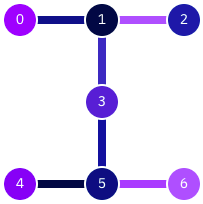
\includegraphics[scale=0.6]{ibmqJakarta.png}
      \caption{Connectivity of \textit{ibmq jakarta} processor. Taken from the official IBM Quantum site.}
      \label{fig:JakartaConnectivity}
    \end{figure}

    Experiments involving direct transpilation and gate-efficient schemes, are performed using qubits 0, 1, and 2. While experiments involving pulse-efficient schemes are performed on qubits 1, 3, and 5. Quantum devices are calibrated each day, and may vary. However, typical parameter values are reported on table \ref{tab:jakartaParams}.

    \begin{table}{H}
      \begin{center}
        \begin{tabular}{| c | c |}
          \hline 
          $T_1$ & 130 $\mu$s \\
          \hline
          $T_2$ & 34 $\mu$s \\
          \hline
          $\epsilon_{\text{CNOT}}$ & 1\% \\
          \hline
          $\epsilon_{\text{Read}}$ & 2\% \\
          \hline
        \end{tabular}
      \end{center}
      \caption{Typical parameter values for \textit{ibmq jakarta}. The coherence times are discussed on the previous chapter. $\epsilon_O$ denotes the error on performing an operation $O$. In this case, CNOT gates and readout.}
      \label{tab:jakartaParams}
    \end{table}

%%%%%%%%%%%%%%%%%%%%%%%%%%%%%%%%%%%%%%%%%%%%%%%%%%%%%%%%%%%%%%%%%%%%%%%%%%%%%%%%